\documentclass[12pt,a4paper]{article}
\usepackage{amsmath}
\usepackage{amsfonts}
\usepackage{amssymb}
\usepackage[utf8]{inputenc}
\usepackage[T1,T2A]{fontenc}
\usepackage[english, russian]{babel}
\usepackage{graphicx}
\usepackage[left=2cm,right=2cm,top=2cm,bottom=2cm]{geometry}
\usepackage{calc}
\usepackage{wrapfig}
\usepackage{setspace}
\usepackage{indentfirst}
\usepackage{subfigure}
\usepackage{afterpage}
\usepackage{comment}
\setlength\parindent{0pt}

\title{
Отчет о выполнении лабораторной работы 2.2.2 \\
Измерение теплопроводности воздуха при разных давлениях
}

\author{Фокин Алексей, 2-922 группа}

\begin{document}
\maketitle

\paragraph{Цель работы:} исследовать теплопередачу от нагретой нити к цилиндрической оболочке в зависимости от концентрации (давления) заполняющего её воздуха. Измерить коэффициент теплопроводности при высоких давлениях; определить область перехода к режиму теплопередачи; определить коэффициент теплопередачи при низких давлениях.
\paragraph{В работе используются:}цилиндрическая колба с натянутой по оси платиновой нитью; форвакуумный насос; вакуумметр; масляный манометр; вольтметр и амперметр (цифровые мультиметры); источник постоянного тока.

\section{Теоретическая справка}
	Теплопроводность — это процесс передачи энергии от нагретых частей системы к холодным за счёт хаотического движения частиц среды (молекул, атомов и т.п.). В газах теплопроводность осуществляется за счёт непосредственной передачи кинетической энергии от быстрых молекул к медленным при их столкновениях. Перенос тепла описывается законом Фурье:
	\begin{equation}
		\vec{q} = -\varkappa\cdot\nabla T,
	\end{equation}
	где $\vec{q}$ --- плотность потока энергии, $\varkappa$ --- коэффициент теплопроводности. Система, используемая в данной установке, имеет цилиндрическую симметрию (пренебрегая краевым эффектами), поэтому имеем 
	\begin{equation}
		q = -\varkappa\frac{dT}{dr},
	\end{equation}
	где $r$ --- расстояние от оси симметрии системы.
	
	Закон Фурье применим при условиях $$\lambda\ll r\quad \text{и}\quad \lambda |\nabla T|\ll T, $$
	где $\lambda$--- длина свободного пробега молекул газа, а $r$--- характерный размер системы.
	
	Для количественного описания способности некоторой системы к теплопередаче в целом используют коэффициент $K$, называемый \emph{тепловым сопротивлением}, равный отношению перепада температур $\Delta T$ в системе к полному потоку энергии $Q$ [Вт] через неё:
	\begin{equation}
		K = \frac{\Delta T}{Q}
	\end{equation}
	
	
	
	\paragraph{Режим теплопроводности} реализуется при выполнении условий выше. Молекулярно-кинетическая теория даёт следующую оценку для коэффициента теплопроводности:
	\begin{equation}
	\varkappa \approx \frac{1}{3}\lambda\bar{v}nc_V,
	\end{equation}
	где $n$ --- концентрация молекул газа, $\bar{v}$ --- их средняя тепловая скорость, $c_V = \frac{i}{2}k$ --- теплоёмкость при постоянном объёме в расчёте на одну молекулу.
	
	Длина свободного пробега обратно пропорциональна n, поэтому коэффициент теплопроводности газа (5) не зависит от его концентрации (т. е. и от давления) и определяется только его температурой.
	
	
	
	\paragraph{Режим теплопередачи.} В случае $\lambda \gtrsim r$ молекулы сталкиваются в основном не между собой, а со стенками. При этом теряет смысл понятие температуры как функции координат и, следовательно, градиента температуры, так что закон Фурье (1) становится неприменим. Если в системе есть поверхности, находящиеся при разных температурах, процесс обмена энергией между ними за счёт молекул газа, заполняющего сосуд, принято называть теплопередачей. Молекулы при неупругих ударах о нагретую поверхность приобретают среднюю кинетическую энергию, соответствующую температуре этой поверхности; отразившись от неё и не сталкиваясь с другими молекулами, они долетают до холодной поверхности и передают ей избыточную энергию.\\
	
	Рассмотрим упрощённую модель теплопередачи в цилиндрическом сосуде радиуса $R$ и длины $L\gg R$, на оси которого натянута тонкая нить радиуса $r\ll R$. Температуры колбы и нити равны $T_\text{к}$ и $T_\text{н} > T_\text{к}$.
	Все молекулы в пространстве колбы можно разделить на две группы: в зависимости от того, с какой поверхностью --- с колбой или с нитью --- они испытали последнее неупругое столкновение, их средняя энергия равна $c_V T_\text{к}$ либо $c_V T_\text{н}$ соответственно. В стационарном состоянии потоки частиц, падающих на нить и улетающих от неё, равны. Тогда полный поток падающих на нить частиц составляет
	$$J = \frac{1}{4}n\bar{v}S_\text{н},$$
	где $S_\text{н} = 2\pi r_\text{н} L$ --- площадь поверхности нити. В нашей работе относительный перепад температур мал ($\Delta T \ll T$), поэтому при расчёте потока частиц можно не различать средние скорости «горячих» (летящих от нити) и «холодных» (летящих к нити) частиц.\\
	
	Если учесть, что не все столкновения молекул с нитью или стенками колбы являются неупругими, введя поправочный множитель $s$, называемый коэффициентом аккомодации, который в наших условиях можно считать постоянным, суммарный поток энергии от нити к колбе может быть приближённо записан как $$Q \approx \frac{s}{4} n \bar{v} S_{\text{н}} \cdot c_{V}\left(T_{\text{н}}-T_{\text{к}}\right)$$
	И тогда
	\begin{equation}
	\frac{1}{K_T}=\frac{s}{4} \bar{v} n c_{V} S_{\text{н}}
	\end{equation}
	
	
	
	\paragraph{Общий случай.} Таким образом, при больших n будет реализоваться случай теплопроводности, а при маленьких --- теплопередачи. Пусть через нить пропускают постоянный ток, так что на ней выделяется известная мощность $Q$. В стационарном состоянии полный поток энергии через любую цилиндрическую поверхность радиуса $r$ должен быть одинаков и равен $Q$. 
	
	\textbf{В области теплопроводности} из (2) имеем
	\begin{equation}
	Q=-2 \pi r L \cdot x \frac{d T}{d r}=\text { const. }\left(r_{\text{н}}+\lambda \lesssim r \leq R\right)
	\end{equation}
	
	\begin{wrapfigure}{r}{60mm}
		\centering
		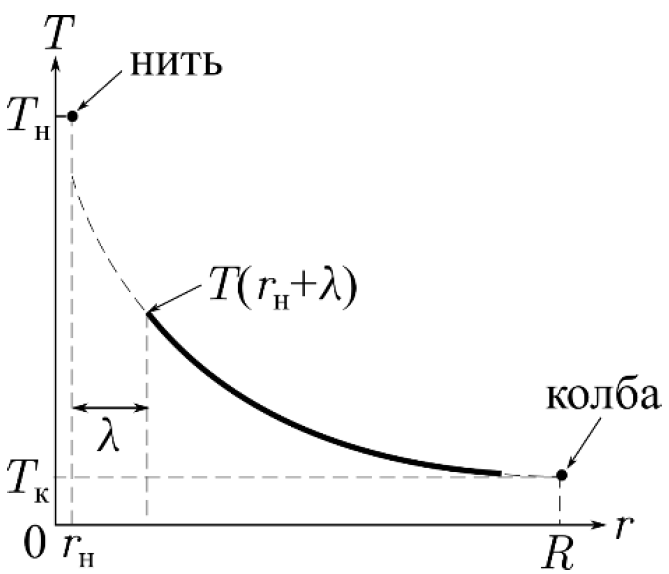
\includegraphics[width=55mm]{C:/Users/ПК/Desktop/Учеба/Лабы/Терма/2.2.2/Тем}
		\caption{Распределение температуры в цилиндре}\small
		\label{fig:}
	\end{wrapfigure}

	Если перепад температуры между стенками колбы и нитью мал, при интегрировании (8) можно пренебречь зависимостью теплопроводности от температуры. Тогда получим
	\begin{equation}
	T(r)-T_{\text{н}}=\frac{Q}{2 \pi L\varkappa} \ln \frac{R}{r}
	\end{equation}
	
	\textbf{В области вблизи нити} ($r_\text{н} \leqslant r \lesssim r_\text{н} + \lambda$) имеем
	\begin{equation}
	T_\text{н} - T(r_\text{н} + \lambda) = K_T Q,
	\end{equation}
	где $K_T$ — тепловое сопротивление области теплопередачи, определяемое формулой (5), $T(r_\text{н} + \lambda)$ — температура газа на границе этой области. Подставив в (7) $r = r_\text{н} + \lambda$ и, исключив с помощью (8) промежуточную температуру $T(r_\text{н} + \lambda)$, найдём разность температур нити и колбы:
	\begin{equation}
	\Delta T=Q\left(\frac{1}{2 \pi L \varkappa} \ln \frac{R}{r_{\text{н}}+\lambda}+K_{T}\right)
	\end{equation}
	С учётом (4) и (5) можно получить явную зависимость от концентрации.
	\begin{equation}
	\Delta T = 
	\frac{Q}{2 \pi L} \left( 
	\frac{1}{\varkappa}\ln \frac{R}{r_{\text{н}}} - 
	\frac{1}{\varkappa}\ln \left(1 + \frac{1}{n\sigma\cdot r_\text{н}}\right) + 
	\frac{1}{\frac{s}{4} r_{\text{н}} \bar{v} c_{V}} \cdot \frac{1}{n} \right)
	\end{equation}
	Нетрудно видеть, что второе слагаемое, с одной стороны, мало при больших давлениях; с другой стороны, при малых давлениях слабая логарифмическая зависимость будет незаметна на фоне слагаемого $K_T$, возрастающего, согласно (5). Поэтому в указанных пределах можно принять, что $\ln \frac{R}{r_{\text{н}}+\lambda} \approx \ln \frac{R}{r_{\text{н}}}$. Учитывая, что непосредственно измеряемой в опыте величиной является давление $P$, можно представить (9) в следующем максимально упрощённом виде:
	\begin{equation}
	\Delta T = Q\left(K_\infty + \frac{A}{P}\right),
	\end{equation}
	где $K_\infty$ и $A$ — константы, которые могут быть определены экспериментально. Величина $K_\infty$ есть тепловое сопротивление системы при высоких давлениях, по его значению может быть вычислен коэффициент теплопроводности газа $\varkappa$. По значению коэффициента $A$ можно определить коэффициент аккомодации $s$.



\subsection*{Экспериментальная установка}
	\begin{figure}
		\centering
		\includegraphics[width=80mm]{C:/Users/ПК/Desktop/Учеба/Лабы/Терма/2.2.2/У}
		\caption{Вакуумная часть установки}
		\label{fig:}
	\end{figure}
	Схема установки приведена на рис. 2. Внутренняя полость тонкостенной цилиндрической стеклянной колбы, на оси которой натянута металлическая (платиновая) нить, подсоединена к вакуумной установке. Колба заполнена воздухом и расположена вертикально. Контактные провода от нити выведены наружу через стеклянную вакуумную «слёзку».
	
	Вакуумная установка состоит из форвакуумного насоса, стрелочного вакуумметра $M$ и U-образного масляного манометра. Вакуумметр служит для измерения высоких давлений вплоть до ~10 торр (он показывает разность давлений между установкой и атмосферой, так что нуль на его шкале соответствует атмосферному давлению в установке). U-образный манометр заполнен маслом с плотностью 0,885 г/см$^3$ и предназначен для измерения низких давлений (вплоть до ~0,1 торр). Кран К$_1$ служит для соединения установки и насоса с атмосферой, кран К$_2$ — для отсоединения откачиваемого объёма от насоса, кран К$_3$ — для соединения колен U-образного манометра.
	
	Металлическая нить служит как источником тепла, так и датчиком температуры (термометром сопротивления). В рабочем диапазоне температур (20–40 $^\circ C$) сопротивление платины зависит от температуры практически линейно:
	\begin{equation}
	R(t)=R_{0}\left(1+\alpha_{0} t\right)
	\end{equation}
	где $t$ --- температура в $^\circ C$, $R_0$--- сопротивление про 0$^\circ C$, и
	\begin{equation}
	\alpha_{0}=\frac{1}{R_{0}} \frac{d R}{d t}=3,92 \cdot 10^{-3} ~^\circ C^{-1}
	\end{equation}
	
	\begin{wrapfigure}{r}{50mm}
		\centering
		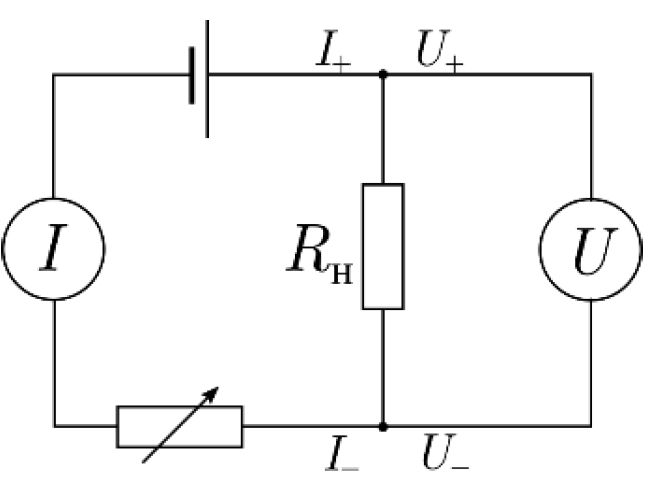
\includegraphics[width=50mm]{C:/Users/ПК/Desktop/Учеба/Лабы/Терма/2.2.2/Элсхема}
		\caption{Электрическая схема измерений}
		\label{fig:}
	\end{wrapfigure}

	Электрическая схема установки приведена на рис. 3. Ток $I$ через сопротивление $R_\text{н}$ и напряжение $U$ на нём измеряются цифровыми мультиметрами, один из которых работает в режиме амперметра, а другой — вольтметра. Сопротивление $R_\text{н}$ находится по закону Ома. Те же измерения позволяют определить мощность нагрева проволоки как джоулево тепло. Ток в цепи регулируется с помощью магазина сопротивлений, включённого последовательно с источником тока.
	
	
	
	\paragraph{Методика измерений.} 
	Поскольку относительное изменение сопротивления невелико ($\Delta R_\text{н}/R_\text{н} \approx 0,4\%   $ при $\Delta T = 1 ^\circ C$), измерение $R_\text{н}$ важно провести с хорошей точностью. Это возможно с помощью построения нагрузочной кривой — зависимости измеряемого сопротивления от выделяющейся в нём мощности $R(Q)$. В данной работе проводится серия измерений перегрева нити относительно стенок сосуда $\Delta T$ в зависимости от мощности нагрева $Q$ при различных давлениях $P$ в системе. Посредством аппроксимации зависимостей  $\Delta T(Q)$ прямыми линиями, определяется полное тепловое сопротивление системы $K = \frac{dT}{dQ}$ при разных $P$. Проверяется справедливость зависимости (10) и определяются коэффициенты $A$ и $K_\infty$, из которых находятся значения коэффициента теплопроводности воздуха $\varkappa$ при высоких давлениях и значение коэффициента аккомодации $s$.\\
	
	Два обстоятельства, которые могут привести к нарушению зависимости (10) --- это остаточное давление воздуха, десорбирующегося из масляного манометра, а также давление паров самого масла и охлаждение нити за счёт излучения. Первое обстоятельство приводит к тому, что измеряемое давление оказывается меньше реального на некоторую неизвестную величину $P_\text{ост}$, что особенно заметно проявляется при малых $P$. Мощность же, излучаемая с поверхности нити, может быть найдена по закону Стефана–Больцмана:
	\begin{equation}
	Q_{\text {изл}}=\epsilon S_{\text{н}} \sigma_{S}\left(T_{\text{н}}^{4}-T_{\text{к}}^{4}\right) \approx 4 \epsilon S_{\text{н}} \sigma_{S} T_{\text{k}}^{3} \Delta T
	\end{equation}
	где $\sigma_S = 5,67\cdot 10^{-8}~\text{Вт/(м}^2\text{К}^4),\ \epsilon = 0,04$. Численно получаем, что на давлениях до $\sim 10^{-1}$ излучением можно пренебречь.
\section{Ход работы}
	\begin{enumerate}
		\item Зафиксируем параметры установки: $$2r_\text{н} = 0,05~\text{мм}\quad 2R = 10~\text{мм} \quad L = 220~\text{мм}$$
		\item Оценим, когда длина свободного пробега примерно сравнивается с радиусом нити: $$
		\lambda (P_1) \approx r_\text{н} \quad
		\Leftrightarrow \quad
		P_1 \approx \frac{kT}{r_\text{н}\pi d^2} \approx 500~\text{мм. масл. ст.}
		$$
		\item Снимаем значение атмосферного давления и температуры в комнате: $$P = 99600~\text{Па} \quad T_\text{к} = 297,3 ~\text{К}$$
		\item Проверяем, что установка находится под вакуумом (стрелка вакуумметра в положении <<-1 атм>>).
		\item Плавно запускаем воздух в установку, медленно открывая кран К$_2$.
		\item Включаем в сеть цифровые мультиметры. Устанавливаем амперметр в режим измерения постоянного тока, а вольтметр — постоянного напряжения. На магазине сопротивлений устанавливаем значение 1 кОм.
		\item Строим нагрузочную кривую при атмосферном давлении, данные приводим на графике (рис. 4)
		%%табл
		\begin{figure}[h!]
			\centering
			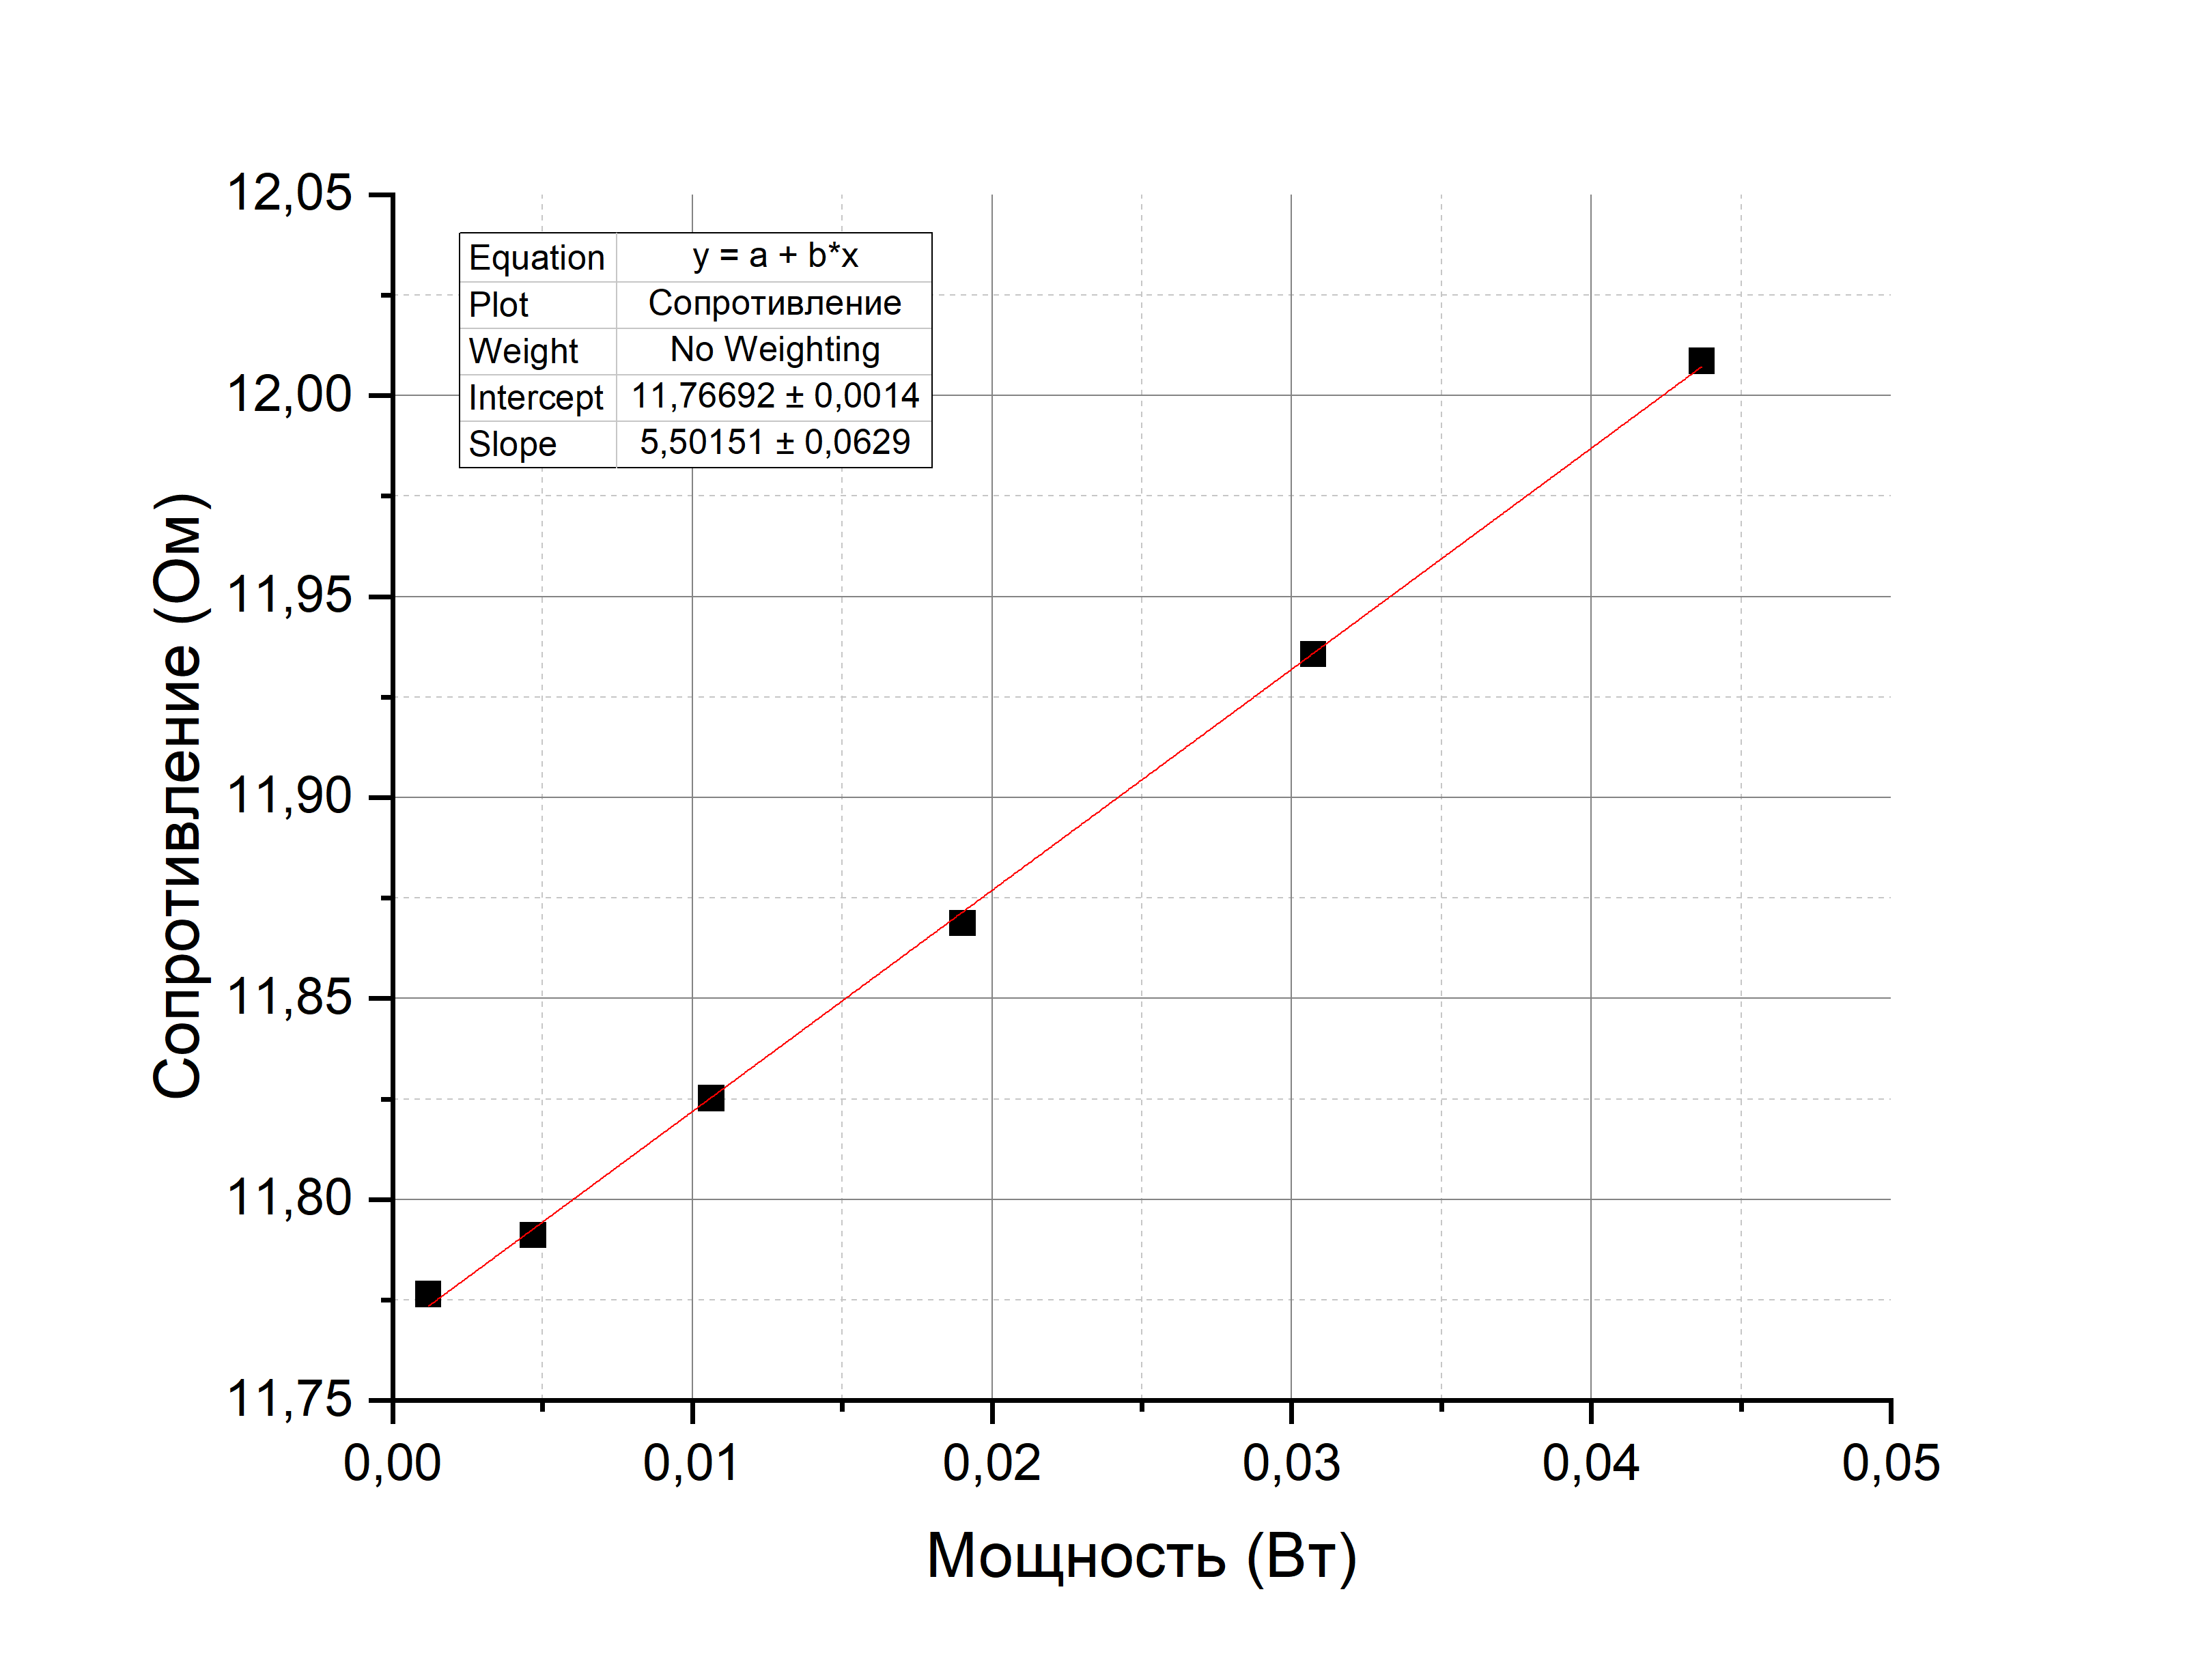
\includegraphics[width=0.7\linewidth]{../../../../../../Users/ПК/Desktop/Учеба/Лабы/Терма/2.2.2/Атмосфера}
			\caption{Нагрузочная кривая при атмосферном давлении}
			\label{fig:}
		\end{figure}
		\item Экстраполируя к нулевому значению мощности, определяем: 
		$$R_\text{к} = (11, 767 \pm 0,002) ~\text{Ом}, \quad R_0 = (10,750 \pm 0,002) ~\text{Ом},\quad R_{max} = (13,037 \pm 0,002) ~\text{Ом}$$
		где $R_\text{к}$ --- сопротивление нити при комнатной температуре, $R_0$ --- сопротивление при $0 ^\circ C$ (по формуле (11)), $R_{max}$ --- соответствующее нагреву нити относительно стенок на $30 ^\circ C$ сопротивление.
		\item Откачиваем установку до предельного вакуума, предварительно откачав насос при закрытых на 20 секунд К$_1$ и К$_2$, в течение 15 минут.
		\item Приводим в действие масляный манометр, проверяя по нему, что давление больше не меняется.
		\item Отсоединяем насос, выключаем его и соединяем его с атмосферой.
		\item Проводим аналогичные пункту 6 измерения в диапазоне $P_{min} \lesssim P \lesssim P_1$: \\
		\emph{см. рис. 5 и табл. 1}
		
		\item Проводим аналогичные пункту 6 измерения в диапазоне $P_1 \lesssim P \lesssim P_{\text{атм}}$:\\
		\emph{см. рис. 6 и табл. 2}
		\afterpage{
				\begin{table}[p] %данные низкие давления
					\centering
					\resizebox{0.8\textwidth}{!}{%
						\begin{tabular}{lllllllllll}
							\cline{1-5} \cline{7-11}
							\multicolumn{5}{|c|}{40 мм масл. ст.} &
							\multicolumn{1}{l|}{} &
							\multicolumn{5}{c|}{80 мм масл. ст.} \\ \cline{1-5} \cline{7-11} 
							\multicolumn{1}{|l|}{U, mV} &
							\multicolumn{1}{l|}{I, mA} &
							\multicolumn{1}{l|}{R, Ом} &
							\multicolumn{1}{l|}{N, Вт} &
							\multicolumn{1}{l|}{T, K} &
							\multicolumn{1}{l|}{} &
							\multicolumn{1}{l|}{U, mV} &
							\multicolumn{1}{l|}{I, mA} &
							\multicolumn{1}{l|}{R, Ом} &
							\multicolumn{1}{l|}{N, Вт} &
							\multicolumn{1}{l|}{T, K} \\ \cline{1-5} \cline{7-11} 
							\multicolumn{1}{|l|}{123,41} &
							\multicolumn{1}{l|}{10,52} &
							\multicolumn{1}{l|}{11,73099} &
							\multicolumn{1}{l|}{0,001298} &
							\multicolumn{1}{l|}{296,4454} &
							\multicolumn{1}{l|}{} &
							\multicolumn{1}{l|}{117,43} &
							\multicolumn{1}{l|}{10,003} &
							\multicolumn{1}{l|}{11,73948} &
							\multicolumn{1}{l|}{0,001175} &
							\multicolumn{1}{l|}{296,6469} \\ \cline{1-5} \cline{7-11} 
							\multicolumn{1}{|l|}{241,23} &
							\multicolumn{1}{l|}{20,5} &
							\multicolumn{1}{l|}{11,76732} &
							\multicolumn{1}{l|}{0,004945} &
							\multicolumn{1}{l|}{297,3075} &
							\multicolumn{1}{l|}{} &
							\multicolumn{1}{l|}{236,22} &
							\multicolumn{1}{l|}{20} &
							\multicolumn{1}{l|}{11,811} &
							\multicolumn{1}{l|}{0,004724} &
							\multicolumn{1}{l|}{298,3442} \\ \cline{1-5} \cline{7-11} 
							\multicolumn{1}{|l|}{364,75} &
							\multicolumn{1}{l|}{30,86} &
							\multicolumn{1}{l|}{11,81951} &
							\multicolumn{1}{l|}{0,011256} &
							\multicolumn{1}{l|}{298,5461} &
							\multicolumn{1}{l|}{} &
							\multicolumn{1}{l|}{353,19} &
							\multicolumn{1}{l|}{29,92} &
							\multicolumn{1}{l|}{11,80448} &
							\multicolumn{1}{l|}{0,010567} &
							\multicolumn{1}{l|}{298,1894} \\ \cline{1-5} \cline{7-11} 
							\multicolumn{1}{|l|}{480,7} &
							\multicolumn{1}{l|}{40,46} &
							\multicolumn{1}{l|}{11,88087} &
							\multicolumn{1}{l|}{0,019449} &
							\multicolumn{1}{l|}{300,0023} &
							\multicolumn{1}{l|}{} &
							\multicolumn{1}{l|}{479,26} &
							\multicolumn{1}{l|}{40,42} &
							\multicolumn{1}{l|}{11,857} &
							\multicolumn{1}{l|}{0,019372} &
							\multicolumn{1}{l|}{299,4359} \\ \cline{1-5} \cline{7-11} 
							\multicolumn{1}{|l|}{600,83} &
							\multicolumn{1}{l|}{50,17} &
							\multicolumn{1}{l|}{11,97588} &
							\multicolumn{1}{l|}{0,030144} &
							\multicolumn{1}{l|}{302,2571} &
							\multicolumn{1}{l|}{} &
							\multicolumn{1}{l|}{598,05} &
							\multicolumn{1}{l|}{50,12} &
							\multicolumn{1}{l|}{11,93236} &
							\multicolumn{1}{l|}{0,029974} &
							\multicolumn{1}{l|}{301,2243} \\ \cline{1-5} \cline{7-11} 
							\multicolumn{1}{|l|}{727,14} &
							\multicolumn{1}{l|}{60,23} &
							\multicolumn{1}{l|}{12,07272} &
							\multicolumn{1}{l|}{0,043796} &
							\multicolumn{1}{l|}{304,5553} &
							\multicolumn{1}{l|}{} &
							\multicolumn{1}{l|}{725,24} &
							\multicolumn{1}{l|}{59,7} &
							\multicolumn{1}{l|}{12,14807} &
							\multicolumn{1}{l|}{0,043297} &
							\multicolumn{1}{l|}{306,3436} \\ \cline{1-5} \cline{7-11} 
							&
							&
							&
							&
							&
							&
							&
							&
							&
							&
							\\
							&
							&
							&
							&
							&
							&
							&
							&
							&
							&
							\\ \cline{1-5} \cline{7-11} 
							\multicolumn{5}{|c|}{112 мм масл. ст.} &
							\multicolumn{1}{l|}{} &
							\multicolumn{5}{c|}{145 мм масл. ст.} \\ \cline{1-5} \cline{7-11} 
							\multicolumn{1}{|l|}{U, mV} &
							\multicolumn{1}{l|}{I, mA} &
							\multicolumn{1}{l|}{R, Ом} &
							\multicolumn{1}{l|}{N, Вт} &
							\multicolumn{1}{l|}{T, K} &
							\multicolumn{1}{l|}{} &
							\multicolumn{1}{l|}{U, mV} &
							\multicolumn{1}{l|}{I, mA} &
							\multicolumn{1}{l|}{R, Ом} &
							\multicolumn{1}{l|}{N, Вт} &
							\multicolumn{1}{l|}{T, K} \\ \cline{1-5} \cline{7-11} 
							\multicolumn{1}{|l|}{107,18} &
							\multicolumn{1}{l|}{9,126} &
							\multicolumn{1}{l|}{11,74447} &
							\multicolumn{1}{l|}{0,000978} &
							\multicolumn{1}{l|}{296,7652} &
							\multicolumn{1}{l|}{} &
							\multicolumn{1}{l|}{117,755} &
							\multicolumn{1}{l|}{10,013} &
							\multicolumn{1}{l|}{11,76021} &
							\multicolumn{1}{l|}{0,001179} &
							\multicolumn{1}{l|}{297,1389} \\ \cline{1-5} \cline{7-11} 
							\multicolumn{1}{|l|}{236,652} &
							\multicolumn{1}{l|}{20,1} &
							\multicolumn{1}{l|}{11,77373} &
							\multicolumn{1}{l|}{0,004757} &
							\multicolumn{1}{l|}{297,4597} &
							\multicolumn{1}{l|}{} &
							\multicolumn{1}{l|}{236,869} &
							\multicolumn{1}{l|}{20,11} &
							\multicolumn{1}{l|}{11,77867} &
							\multicolumn{1}{l|}{0,004763} &
							\multicolumn{1}{l|}{297,5769} \\ \cline{1-5} \cline{7-11} 
							\multicolumn{1}{|l|}{353,934} &
							\multicolumn{1}{l|}{29,97} &
							\multicolumn{1}{l|}{11,80961} &
							\multicolumn{1}{l|}{0,010607} &
							\multicolumn{1}{l|}{298,3112} &
							\multicolumn{1}{l|}{} &
							\multicolumn{1}{l|}{354,31} &
							\multicolumn{1}{l|}{29,99} &
							\multicolumn{1}{l|}{11,81427} &
							\multicolumn{1}{l|}{0,010626} &
							\multicolumn{1}{l|}{298,4218} \\ \cline{1-5} \cline{7-11} 
							\multicolumn{1}{|l|}{478,1} &
							\multicolumn{1}{l|}{40,26} &
							\multicolumn{1}{l|}{11,87531} &
							\multicolumn{1}{l|}{0,019248} &
							\multicolumn{1}{l|}{299,8704} &
							\multicolumn{1}{l|}{} &
							\multicolumn{1}{l|}{480,815} &
							\multicolumn{1}{l|}{40,49} &
							\multicolumn{1}{l|}{11,87491} &
							\multicolumn{1}{l|}{0,019468} &
							\multicolumn{1}{l|}{299,8608} \\ \cline{1-5} \cline{7-11} 
							\multicolumn{1}{|l|}{601,1} &
							\multicolumn{1}{l|}{50,31} &
							\multicolumn{1}{l|}{11,94792} &
							\multicolumn{1}{l|}{0,030241} &
							\multicolumn{1}{l|}{301,5936} &
							\multicolumn{1}{l|}{} &
							\multicolumn{1}{l|}{599,851} &
							\multicolumn{1}{l|}{50,23} &
							\multicolumn{1}{l|}{11,94209} &
							\multicolumn{1}{l|}{0,030131} &
							\multicolumn{1}{l|}{301,4551} \\ \cline{1-5} \cline{7-11} 
							\multicolumn{1}{|l|}{727,74} &
							\multicolumn{1}{l|}{60,46} &
							\multicolumn{1}{l|}{12,03672} &
							\multicolumn{1}{l|}{0,043999} &
							\multicolumn{1}{l|}{303,7009} &
							\multicolumn{1}{l|}{} &
							\multicolumn{1}{l|}{725,375} &
							\multicolumn{1}{l|}{60,31} &
							\multicolumn{1}{l|}{12,02744} &
							\multicolumn{1}{l|}{0,043747} &
							\multicolumn{1}{l|}{303,4807} \\ \cline{1-5} \cline{7-11} 
							&
							&
							&
							&
							&
							&
							&
							&
							&
							&
							\\
							&
							&
							&
							&
							&
							&
							&
							&
							&
							&
							\\ \cline{1-5} \cline{7-11} 
							\multicolumn{5}{|c|}{187 мм масл. ст.} &
							\multicolumn{1}{l|}{} &
							\multicolumn{5}{c|}{222 мм масл. ст.} \\ \cline{1-5} \cline{7-11} 
							\multicolumn{1}{|l|}{U, mV} &
							\multicolumn{1}{l|}{I, mA} &
							\multicolumn{1}{l|}{R, Ом} &
							\multicolumn{1}{l|}{N, Вт} &
							\multicolumn{1}{l|}{T, K} &
							\multicolumn{1}{l|}{} &
							\multicolumn{1}{l|}{U, mV} &
							\multicolumn{1}{l|}{I, mA} &
							\multicolumn{1}{l|}{R, Ом} &
							\multicolumn{1}{l|}{N, Вт} &
							\multicolumn{1}{l|}{T, K} \\ \cline{1-5} \cline{7-11} 
							\multicolumn{1}{|l|}{117,695} &
							\multicolumn{1}{l|}{10,003} &
							\multicolumn{1}{l|}{11,76597} &
							\multicolumn{1}{l|}{0,001177} &
							\multicolumn{1}{l|}{297,2756} &
							\multicolumn{1}{l|}{} &
							\multicolumn{1}{l|}{117,85} &
							\multicolumn{1}{l|}{10,014} &
							\multicolumn{1}{l|}{11,76852} &
							\multicolumn{1}{l|}{0,00118} &
							\multicolumn{1}{l|}{297,3362} \\ \cline{1-5} \cline{7-11} 
							\multicolumn{1}{|l|}{236,95} &
							\multicolumn{1}{l|}{20,12} &
							\multicolumn{1}{l|}{11,77684} &
							\multicolumn{1}{l|}{0,004767} &
							\multicolumn{1}{l|}{297,5335} &
							\multicolumn{1}{l|}{} &
							\multicolumn{1}{l|}{237,24} &
							\multicolumn{1}{l|}{20,12} &
							\multicolumn{1}{l|}{11,79125} &
							\multicolumn{1}{l|}{0,004773} &
							\multicolumn{1}{l|}{297,8756} \\ \cline{1-5} \cline{7-11} 
							\multicolumn{1}{|l|}{370,555} &
							\multicolumn{1}{l|}{31,33} &
							\multicolumn{1}{l|}{11,82748} &
							\multicolumn{1}{l|}{0,011609} &
							\multicolumn{1}{l|}{298,7353} &
							\multicolumn{1}{l|}{} &
							\multicolumn{1}{l|}{354,71} &
							\multicolumn{1}{l|}{30,01} &
							\multicolumn{1}{l|}{11,81973} &
							\multicolumn{1}{l|}{0,010645} &
							\multicolumn{1}{l|}{298,5513} \\ \cline{1-5} \cline{7-11} 
							\multicolumn{1}{|l|}{472,3} &
							\multicolumn{1}{l|}{39,77} &
							\multicolumn{1}{l|}{11,87579} &
							\multicolumn{1}{l|}{0,018783} &
							\multicolumn{1}{l|}{299,8817} &
							\multicolumn{1}{l|}{} &
							\multicolumn{1}{l|}{477,08} &
							\multicolumn{1}{l|}{40,19} &
							\multicolumn{1}{l|}{11,87061} &
							\multicolumn{1}{l|}{0,019174} &
							\multicolumn{1}{l|}{299,759} \\ \cline{1-5} \cline{7-11} 
							\multicolumn{1}{|l|}{600,97} &
							\multicolumn{1}{l|}{50,32} &
							\multicolumn{1}{l|}{11,94297} &
							\multicolumn{1}{l|}{0,030241} &
							\multicolumn{1}{l|}{301,476} &
							\multicolumn{1}{l|}{} &
							\multicolumn{1}{l|}{601,29} &
							\multicolumn{1}{l|}{50,36} &
							\multicolumn{1}{l|}{11,93983} &
							\multicolumn{1}{l|}{0,030281} &
							\multicolumn{1}{l|}{301,4016} \\ \cline{1-5} \cline{7-11} 
							\multicolumn{1}{|l|}{726,57} &
							\multicolumn{1}{l|}{60,4} &
							\multicolumn{1}{l|}{12,0293} &
							\multicolumn{1}{l|}{0,043885} &
							\multicolumn{1}{l|}{303,525} &
							\multicolumn{1}{l|}{} &
							\multicolumn{1}{l|}{727,78} &
							\multicolumn{1}{l|}{60,53} &
							\multicolumn{1}{l|}{12,02346} &
							\multicolumn{1}{l|}{0,044053} &
							\multicolumn{1}{l|}{303,3862} \\ \cline{1-5} \cline{7-11} 
						\end{tabular}%
					}
					\caption{Измерения и расчеты (низкие давления)}
					\label{tab:my-table}
				\end{table}
				
				\begin{table}[p] %данные высокие давления
					\centering
					\resizebox{0.8\textwidth}{!}{%
						\begin{tabular}{lllllllllll}
							\cline{1-5} \cline{7-11}
							\multicolumn{5}{|c|}{4,5 кПа} &
							\multicolumn{1}{l|}{} &
							\multicolumn{5}{c|}{5,5 кПа} \\ \cline{1-5} \cline{7-11} 
							\multicolumn{1}{|l|}{U, mV} &
							\multicolumn{1}{l|}{I, mA} &
							\multicolumn{1}{l|}{R, Ом} &
							\multicolumn{1}{l|}{N, Вт} &
							\multicolumn{1}{l|}{T, K} &
							\multicolumn{1}{l|}{} &
							\multicolumn{1}{l|}{U, mV} &
							\multicolumn{1}{l|}{I, mA} &
							\multicolumn{1}{l|}{R, Ом} &
							\multicolumn{1}{l|}{N, Вт} &
							\multicolumn{1}{l|}{T, K} \\ \cline{1-5} \cline{7-11} 
							\multicolumn{1}{|l|}{117,72} &
							\multicolumn{1}{l|}{10,01} &
							\multicolumn{1}{l|}{11,76024} &
							\multicolumn{1}{l|}{0,001178} &
							\multicolumn{1}{l|}{297,1396} &
							\multicolumn{1}{l|}{} &
							\multicolumn{1}{l|}{118,3} &
							\multicolumn{1}{l|}{10,06} &
							\multicolumn{1}{l|}{11,75944} &
							\multicolumn{1}{l|}{0,00119} &
							\multicolumn{1}{l|}{297,1207} \\ \cline{1-5} \cline{7-11} 
							\multicolumn{1}{|l|}{236,88} &
							\multicolumn{1}{l|}{20,12} &
							\multicolumn{1}{l|}{11,77336} &
							\multicolumn{1}{l|}{0,004766} &
							\multicolumn{1}{l|}{297,4509} &
							\multicolumn{1}{l|}{} &
							\multicolumn{1}{l|}{236,91} &
							\multicolumn{1}{l|}{20,11} &
							\multicolumn{1}{l|}{11,78071} &
							\multicolumn{1}{l|}{0,004764} &
							\multicolumn{1}{l|}{297,6253} \\ \cline{1-5} \cline{7-11} 
							\multicolumn{1}{|l|}{354,25} &
							\multicolumn{1}{l|}{30} &
							\multicolumn{1}{l|}{11,80833} &
							\multicolumn{1}{l|}{0,010628} &
							\multicolumn{1}{l|}{298,2809} &
							\multicolumn{1}{l|}{} &
							\multicolumn{1}{l|}{354,3} &
							\multicolumn{1}{l|}{30} &
							\multicolumn{1}{l|}{11,81} &
							\multicolumn{1}{l|}{0,010629} &
							\multicolumn{1}{l|}{298,3205} \\ \cline{1-5} \cline{7-11} 
							\multicolumn{1}{|l|}{474,9} &
							\multicolumn{1}{l|}{40,04} &
							\multicolumn{1}{l|}{11,86064} &
							\multicolumn{1}{l|}{0,019015} &
							\multicolumn{1}{l|}{299,5222} &
							\multicolumn{1}{l|}{} &
							\multicolumn{1}{l|}{480,6} &
							\multicolumn{1}{l|}{40,51} &
							\multicolumn{1}{l|}{11,86374} &
							\multicolumn{1}{l|}{0,019469} &
							\multicolumn{1}{l|}{299,5958} \\ \cline{1-5} \cline{7-11} 
							\multicolumn{1}{|l|}{596,51} &
							\multicolumn{1}{l|}{50,01} &
							\multicolumn{1}{l|}{11,92781} &
							\multicolumn{1}{l|}{0,029831} &
							\multicolumn{1}{l|}{301,1164} &
							\multicolumn{1}{l|}{} &
							\multicolumn{1}{l|}{599,6} &
							\multicolumn{1}{l|}{50,27} &
							\multicolumn{1}{l|}{11,92759} &
							\multicolumn{1}{l|}{0,030142} &
							\multicolumn{1}{l|}{301,1111} \\ \cline{1-5} \cline{7-11} 
							\multicolumn{1}{|l|}{720,8} &
							\multicolumn{1}{l|}{60,04} &
							\multicolumn{1}{l|}{12,00533} &
							\multicolumn{1}{l|}{0,043277} &
							\multicolumn{1}{l|}{302,956} &
							\multicolumn{1}{l|}{} &
							\multicolumn{1}{l|}{725,3} &
							\multicolumn{1}{l|}{60,41} &
							\multicolumn{1}{l|}{12,00629} &
							\multicolumn{1}{l|}{0,043815} &
							\multicolumn{1}{l|}{302,9788} \\ \cline{1-5} \cline{7-11} 
							&
							&
							&
							&
							&
							&
							&
							&
							&
							&
							\\
							&
							&
							&
							&
							&
							&
							&
							&
							&
							&
							\\ \cline{1-5} \cline{7-11} 
							\multicolumn{5}{|c|}{10 кПа} &
							\multicolumn{1}{l|}{} &
							\multicolumn{5}{c|}{15 кПа} \\ \cline{1-5} \cline{7-11} 
							\multicolumn{1}{|l|}{U, mV} &
							\multicolumn{1}{l|}{I, mA} &
							\multicolumn{1}{l|}{R, Ом} &
							\multicolumn{1}{l|}{N, Вт} &
							\multicolumn{1}{l|}{T, K} &
							\multicolumn{1}{l|}{} &
							\multicolumn{1}{l|}{U, mV} &
							\multicolumn{1}{l|}{I, mA} &
							\multicolumn{1}{l|}{R, Ом} &
							\multicolumn{1}{l|}{N, Вт} &
							\multicolumn{1}{l|}{T, K} \\ \cline{1-5} \cline{7-11} 
							\multicolumn{1}{|l|}{117,72} &
							\multicolumn{1}{l|}{10,01} &
							\multicolumn{1}{l|}{11,76024} &
							\multicolumn{1}{l|}{0,001178} &
							\multicolumn{1}{l|}{297,1396} &
							\multicolumn{1}{l|}{} &
							\multicolumn{1}{l|}{117,71} &
							\multicolumn{1}{l|}{10,01} &
							\multicolumn{1}{l|}{11,75924} &
							\multicolumn{1}{l|}{0,001178} &
							\multicolumn{1}{l|}{297,1159} \\ \cline{1-5} \cline{7-11} 
							\multicolumn{1}{|l|}{236,86} &
							\multicolumn{1}{l|}{20,11} &
							\multicolumn{1}{l|}{11,77822} &
							\multicolumn{1}{l|}{0,004763} &
							\multicolumn{1}{l|}{297,5663} &
							\multicolumn{1}{l|}{} &
							\multicolumn{1}{l|}{236,42} &
							\multicolumn{1}{l|}{20,1} &
							\multicolumn{1}{l|}{11,76219} &
							\multicolumn{1}{l|}{0,004752} &
							\multicolumn{1}{l|}{297,1858} \\ \cline{1-5} \cline{7-11} 
							\multicolumn{1}{|l|}{354,1} &
							\multicolumn{1}{l|}{29,99} &
							\multicolumn{1}{l|}{11,80727} &
							\multicolumn{1}{l|}{0,010619} &
							\multicolumn{1}{l|}{298,2557} &
							\multicolumn{1}{l|}{} &
							\multicolumn{1}{l|}{354,92} &
							\multicolumn{1}{l|}{29,97} &
							\multicolumn{1}{l|}{11,84251} &
							\multicolumn{1}{l|}{0,010637} &
							\multicolumn{1}{l|}{299,092} \\ \cline{1-5} \cline{7-11} 
							\multicolumn{1}{|l|}{480,16} &
							\multicolumn{1}{l|}{40,5} &
							\multicolumn{1}{l|}{11,8558} &
							\multicolumn{1}{l|}{0,019446} &
							\multicolumn{1}{l|}{299,4074} &
							\multicolumn{1}{l|}{} &
							\multicolumn{1}{l|}{481,34} &
							\multicolumn{1}{l|}{40,48} &
							\multicolumn{1}{l|}{11,89081} &
							\multicolumn{1}{l|}{0,019485} &
							\multicolumn{1}{l|}{300,2382} \\ \cline{1-5} \cline{7-11} 
							\multicolumn{1}{|l|}{599,15} &
							\multicolumn{1}{l|}{50,27} &
							\multicolumn{1}{l|}{11,91864} &
							\multicolumn{1}{l|}{0,030119} &
							\multicolumn{1}{l|}{300,8987} &
							\multicolumn{1}{l|}{} &
							\multicolumn{1}{l|}{600,1} &
							\multicolumn{1}{l|}{50,21} &
							\multicolumn{1}{l|}{11,9518} &
							\multicolumn{1}{l|}{0,030131} &
							\multicolumn{1}{l|}{301,6857} \\ \cline{1-5} \cline{7-11} 
							\multicolumn{1}{|l|}{724,9} &
							\multicolumn{1}{l|}{60,42} &
							\multicolumn{1}{l|}{11,99768} &
							\multicolumn{1}{l|}{0,043798} &
							\multicolumn{1}{l|}{302,7745} &
							\multicolumn{1}{l|}{} &
							\multicolumn{1}{l|}{725,57} &
							\multicolumn{1}{l|}{60,32} &
							\multicolumn{1}{l|}{12,02868} &
							\multicolumn{1}{l|}{0,043766} &
							\multicolumn{1}{l|}{303,5101} \\ \cline{1-5} \cline{7-11} 
							&
							&
							&
							&
							&
							&
							&
							&
							&
							&
							\\
							&
							&
							&
							&
							&
							&
							&
							&
							&
							&
							\\ \cline{1-5}
							\multicolumn{5}{|c|}{25 кПа} &
							&
							&
							&
							&
							&
							\\ \cline{1-5}
							\multicolumn{1}{|l|}{U, mV} &
							\multicolumn{1}{l|}{I, mA} &
							\multicolumn{1}{l|}{R, Ом} &
							\multicolumn{1}{l|}{N, Вт} &
							\multicolumn{1}{l|}{T, K} &
							&
							&
							&
							&
							&
							\\ \cline{1-5}
							\multicolumn{1}{|l|}{117,86} &
							\multicolumn{1}{l|}{10,009} &
							\multicolumn{1}{l|}{11,7754} &
							\multicolumn{1}{l|}{0,00118} &
							\multicolumn{1}{l|}{297,4994} &
							&
							&
							&
							&
							&
							\\ \cline{1-5}
							\multicolumn{1}{|l|}{237,1} &
							\multicolumn{1}{l|}{20,1} &
							\multicolumn{1}{l|}{11,79602} &
							\multicolumn{1}{l|}{0,004766} &
							\multicolumn{1}{l|}{297,9887} &
							&
							&
							&
							&
							&
							\\ \cline{1-5}
							\multicolumn{1}{|l|}{354,46} &
							\multicolumn{1}{l|}{29,97} &
							\multicolumn{1}{l|}{11,82716} &
							\multicolumn{1}{l|}{0,010623} &
							\multicolumn{1}{l|}{298,7277} &
							&
							&
							&
							&
							&
							\\ \cline{1-5}
							\multicolumn{1}{|l|}{480,8} &
							\multicolumn{1}{l|}{40,48} &
							\multicolumn{1}{l|}{11,87747} &
							\multicolumn{1}{l|}{0,019463} &
							\multicolumn{1}{l|}{299,9217} &
							&
							&
							&
							&
							&
							\\ \cline{1-5}
							\multicolumn{1}{|l|}{599,5} &
							\multicolumn{1}{l|}{50,21} &
							\multicolumn{1}{l|}{11,93985} &
							\multicolumn{1}{l|}{0,030101} &
							\multicolumn{1}{l|}{301,4021} &
							&
							&
							&
							&
							&
							\\ \cline{1-5}
							\multicolumn{1}{|l|}{724,42} &
							\multicolumn{1}{l|}{60,28} &
							\multicolumn{1}{l|}{12,01758} &
							\multicolumn{1}{l|}{0,043668} &
							\multicolumn{1}{l|}{303,2468} &
							&
							&
							&
							&
							&
							\\ \cline{1-5}
						\end{tabular}%
					}
					\caption{Измерения и расчёты (высокие давления)}
					\label{tab:my-table}
				\end{table}
		\clearpage
		}
		
		
		\afterpage{
			\begin{figure}[p!]
				\centering
				\caption{Зависимости температуры нити от мощности (в диапазоне низких давлений)}
				\label{fig:lowpressuretemp}
				\includegraphics[width=1\linewidth]{"../../../../../../Users/ПК/Desktop/Учеба/Лабы/Терма/2.2.2/"Эксперимент (низкие)"}
			\end{figure}
			
			\clearpage
		}
		
		\afterpage{
			\begin{figure}[p!]
				\centering
				\caption{Зависимости температуры нити от мощности (в диапазоне высоких давлений)}
				\includegraphics[width=\linewidth]{"../../../../../../Users/ПК/Desktop/Учеба/Лабы/Терма/2.2.2/"Эксперимент (высокие)"}
				\label{fig:--png}
			\end{figure}
		\clearpage
		}
		
		
		
		
		
		
		
		
		
		\newpage
		\item Построим зависимость теплового сопротивления как коэффициентов наклона графиков (рис. 5-6) от давления:
		\begin{table}[h]
			\centering
			\resizebox{\textwidth}{!}{%
				\begin{tabular}{|l|l|l|l|l|l|l|l|l|l|l|l|}
					\hline
					$K$, $^\circ$К/Вт & 190 & 200 & 161 & 150 & 148 & 141 & 141 & 138 & 133 & 154 & 135 \\ \hline
					$\sigma_K$, $^\circ$К/Вт & 4 & 30 & 2 & 2 & 3 & 2 & 2 & 1 & 2 & 11 & 1 \\ \hline
					$P$, Па & 347 & 694 & 971 & 1258 & 1621 & 1925 & 4500 & 5500 & 10000 & 15000 & 25000 \\ \hline
				\end{tabular}%
			}
			\caption{Тепловое сопротивление (из измерений выше) от давления}
			\label{tab:my-table}
		\end{table}
		
		\begin{figure}[!h]
			\centering
			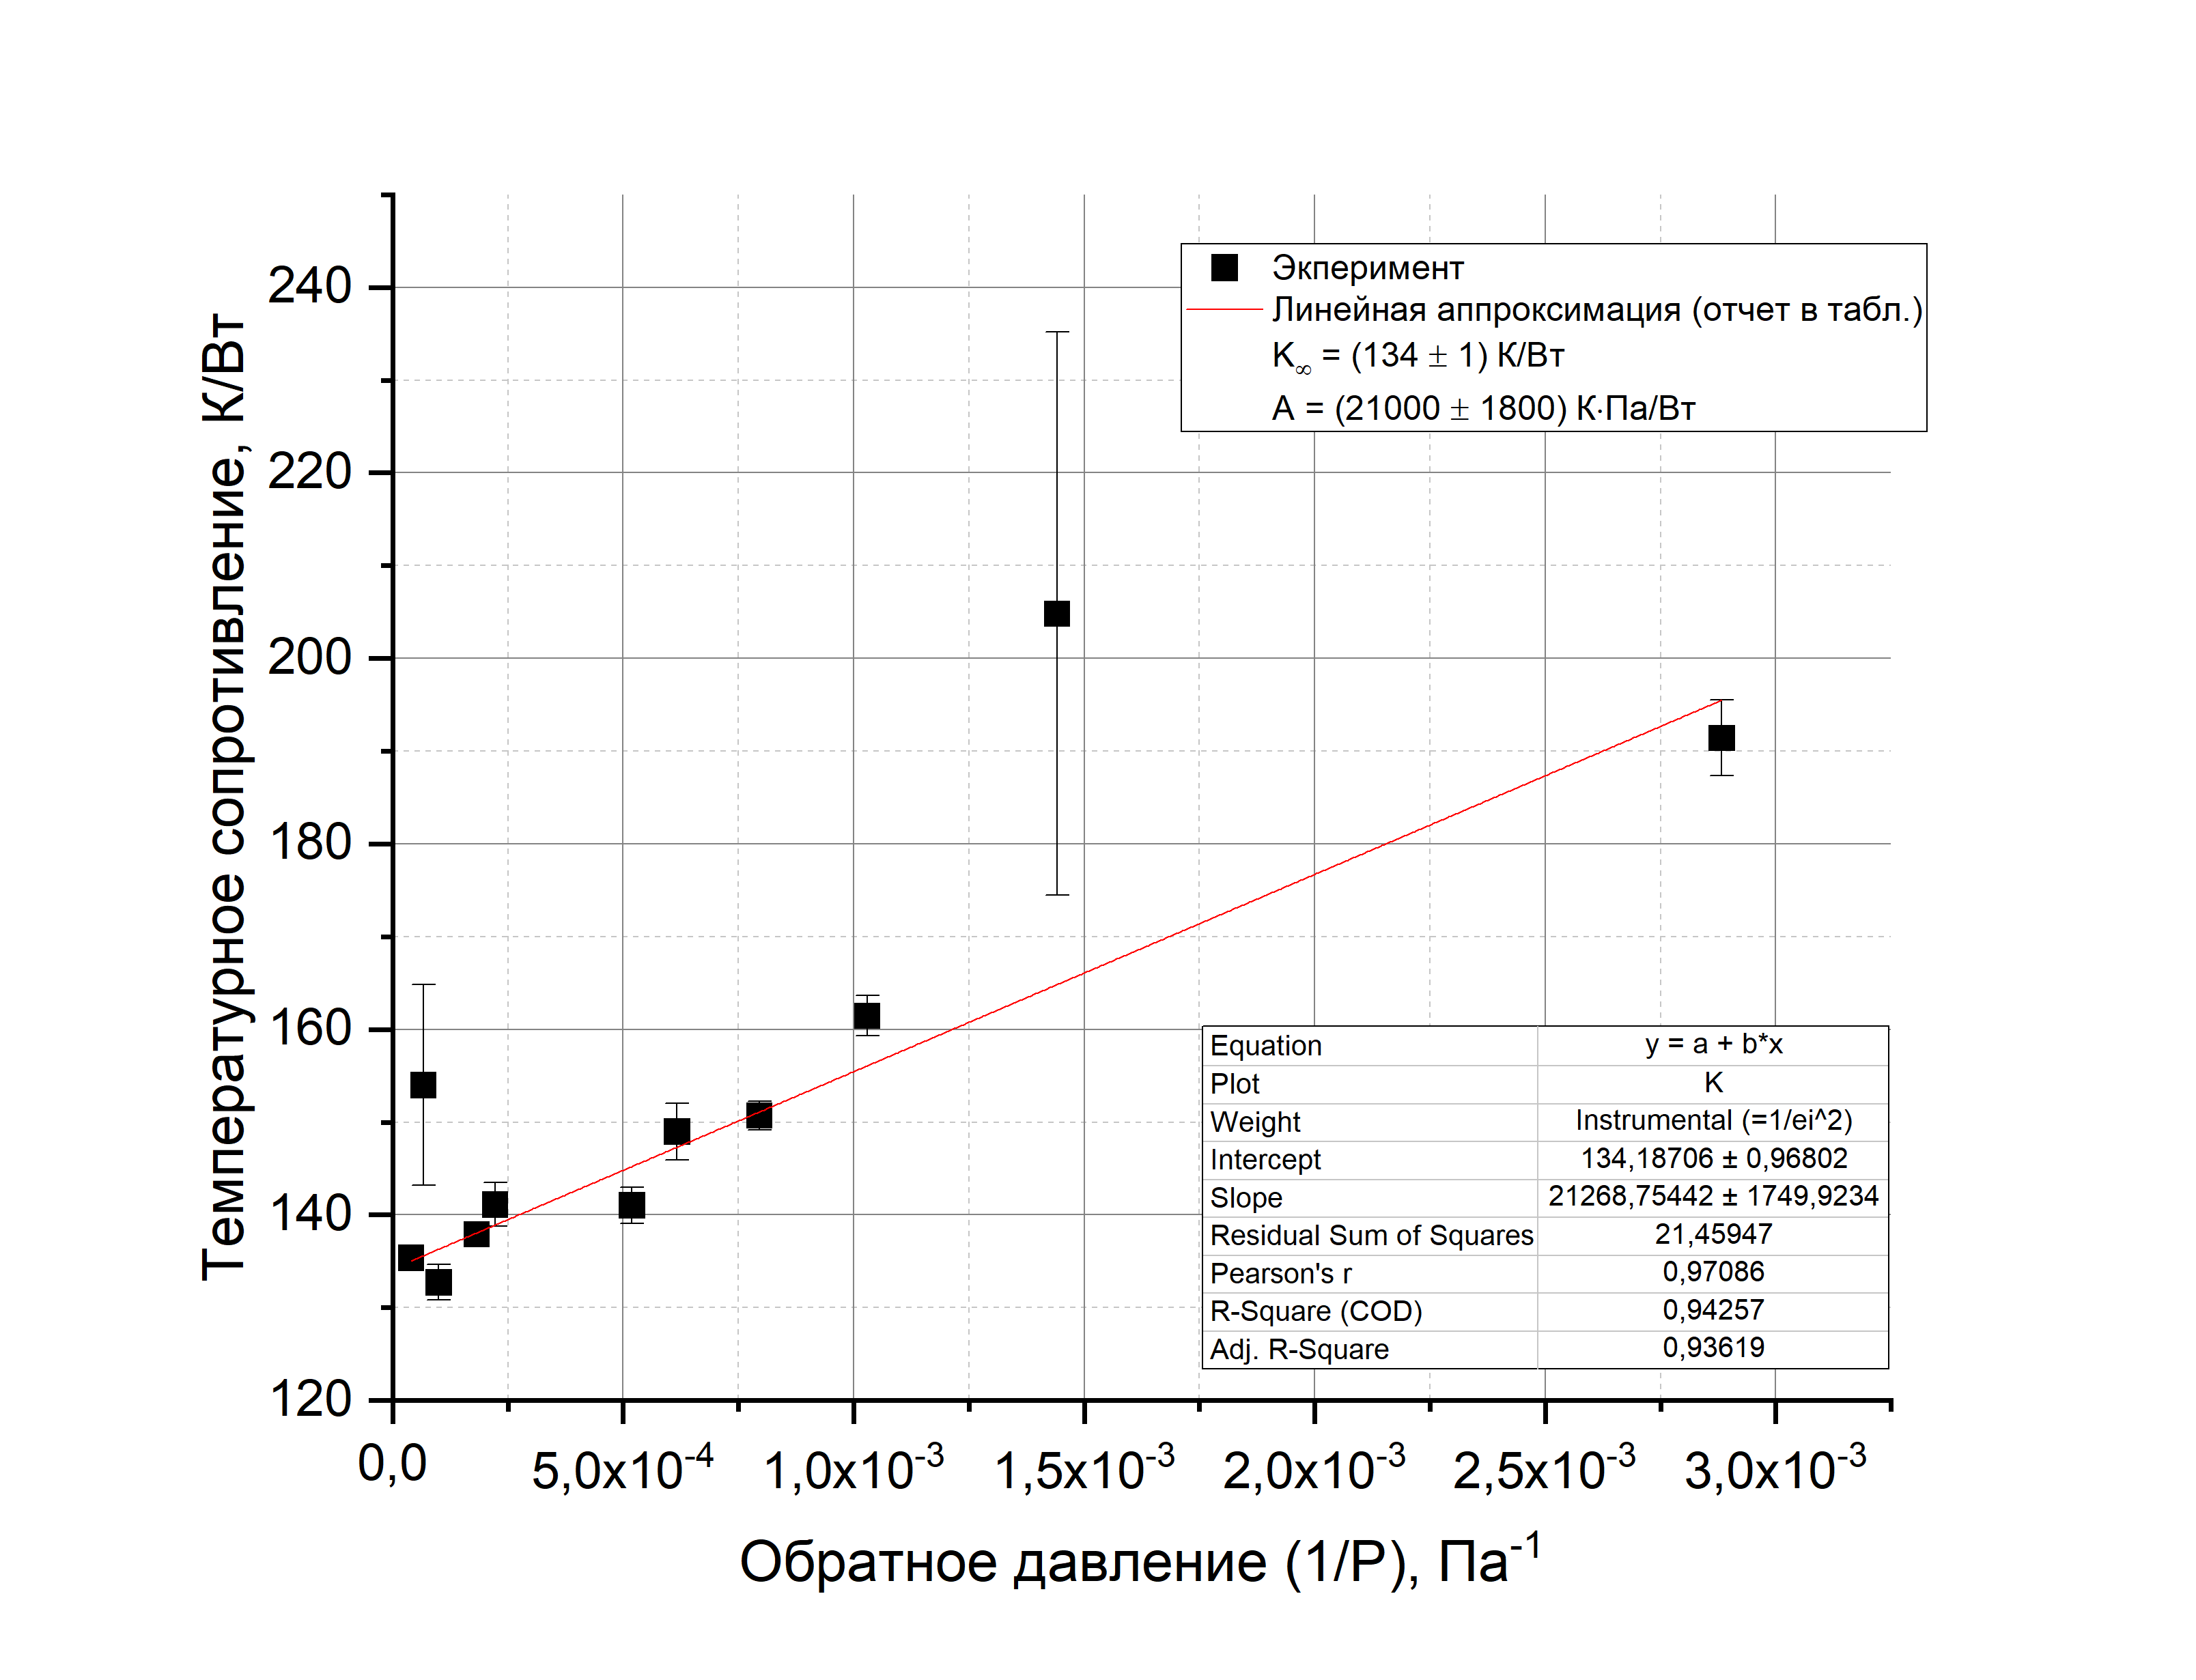
\includegraphics[width=0.7\linewidth]{../../../../../../Users/ПК/Desktop/Учеба/Лабы/Терма/2.2.2/Линия}
			\caption{Зависимость K(1/P)}
			\label{fig:}
		\end{figure}
		\item Получаем коэффициенты в зависимости (10):
		$$A = (21300 \pm 1800) ~\text{К/(Вт}\cdot\text{Па)} \quad K_\infty = (134 \pm 1) ~\text{К/Вт}$$
		\item С помощью (9) можем получить коэффициент теплопроводности воздуха, соответствующий температуре в колбе (мы считали его не зависящим от температуры):
		$$\varkappa = \frac{1}{2\pi L K_\infty} \ln\frac{R}{r_\text{н}} = (28,6 \pm 0,2)\cdot10^{-3} ~\text{Вт/(м}\cdot\text{К)}$$
		А также после преобразований:
		$$s = \frac{1}{Lr_\text{н}C_V\cdot A}\sqrt{\frac{\mu RT_\text{к}}{2\pi}} = 0,70 \pm 0,06 $$
		\item Также проверим теоретическую зависимость в двойном логарифмическом масштабе, построив зависимость $\ln(K - K_\infty)$ от $\ln P$
		\afterpage{
			\begin{figure}
				\centering
				\caption{Зависимость теплового сопротивления от давления в логарифмическом масштабе}
				\includegraphics[width=1\linewidth]{"../../../../../../Users/ПК/Desktop/Учеба/Лабы/Терма/2.2.2/Логафмический масштаб"}
				\label{fig:-}
			\end{figure}
		\clearpage
		}
		
	\end{enumerate}



\newpage
\section{Выводы}
	\begin{enumerate}
	\item В данной работе была проверена предложенная экспериментальная методика по определению коэффициента теплопроводности воздуха при комнатной температуре в зависимости от давления и коэффициента аккомодации.
	\item Были измерены последние с приемлемой точностью.
	\item Была проверена теоретическая зависимость температурного сопротивления газа от давления, которая с некоторой точностью подтвердилась. 
	\end{enumerate}
\end{document}
